\textbf{(DRAFT)} Phonon dispersion and the practical bits of inelastic neutron scattering.
\begin{parts}
	\part BC tetragonal direct lattice $\rightarrow$ FC tetragonal reciprocal lattice\footnote{Proof is similar to the cubic case -- the direct and reciprocal bases no longer share the same length, but they cancel out upon taking $\mathbf{G}\cdot\mathbf{R}$!}.
	
	Also by definition of reciprocal lattice vector, we have:
	\begin{gather*}
		\mathbf{a}^* = \frac{2\pi (\mathbf{b} \times \mathbf{c})}{\mathbf{a} \cdot (\mathbf{b} \times \mathbf{c})} \\
		\Rightarrow a^* = \frac{2\pi}{a} = \SI{16.2}{\per\nano\metre} \\
		\mathbf{c}^* = \frac{2\pi (\mathbf{a} \times \mathbf{b})}{\mathbf{a} \cdot (\mathbf{b} \times \mathbf{c})} \\
		\Rightarrow c^* = \frac{2\pi}{c} = \SI{5.39}{\per\nano\metre}
	\end{gather*}
	
	Taking care of the scaling, we should have the following sketch for $-2 \le h \le 2$ and $-2 \le l \le 2$, together with the 1st BZ shaded:
	\begin{figure}[H]
		\centering
		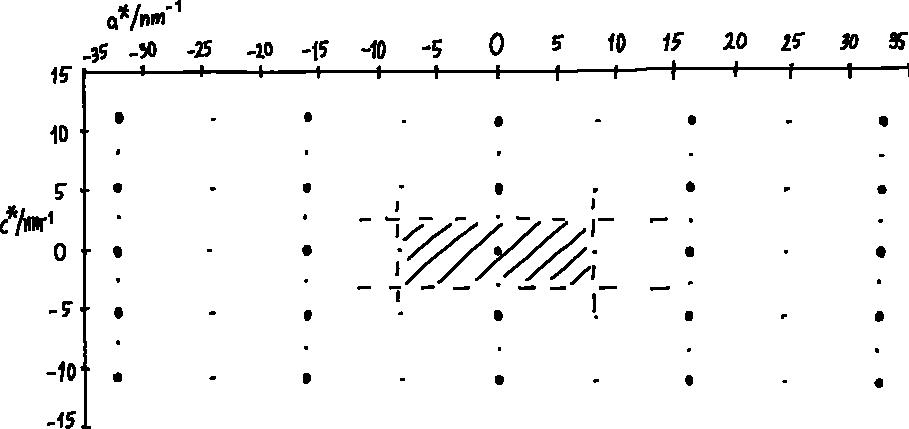
\includegraphics[width=15.5cm]{q6-reciprocal-sketch}
	\end{figure}
	
	\part Questions on phonon dispersion and reciprocal lattice.
	\begin{subparts}
		\subpart For a 3D crystal of $N$ lattice points and $p$ atoms, we have a total of $3Np$ phonon modes.
		
		For CaFe\textsubscript{2}As\textsubscript{2}, $p=5$.
		Hence for a given wavevector, there should be $3p=15$ phonon modes in total.
		
		\subpart \textbf{(TO BE VERIFIED)}
		Note that the positions (1, 0, 0) and (0, 0, 1) are $\Gamma$ points that are symmetry-equivalent by translation.
		Therefore the dispersion curve must meet at those points, i.e. phonon frequencies must be identical.
		
		\subpart Being a tetragonal lattice, the symmetry element 4\textsubscript{z} must be present, hence there will be degenerate transverse modes along the $c$ axis.
		
		Further note that by the definition of acoustic mode in which all atoms oscillate in phase, we'd only have $2$ transverse acoustic (TA) modes which corresponds to vibrations in $a$ and $b$ axes.
		
		Now since the TA modes are degenerate, only $2$ acoustic modes will be observable, with the other one being the longitudinal acoustic (LA) mode.
		
		There is no four-fold rotation symmetry about the $a$ axis, hence all $3$ acoustic modes are non-degenerate.
	\end{subparts}
	
	\part
	\begin{subparts}
		\subpart Definition of scattering vector: $\mathbf{Q} = \mathbf{k}_\textnormal{f} - \mathbf{k}_\textnormal{i} = \mathbf{k}_\textnormal{ph} + \mathbf{G}$ where $\mathbf{k}_\textnormal{ph}$ is the wavevector in the 1st BZ\footnote{It is as if $\mathbf{Q} = \mathbf{k}_\textnormal{ph}  \pmod{\mathbf{G}}$ at a slight abuse of notation.}.
		
		For inelastic neutron scattering, we have the following accessible Ewald sphere by the conservation of momentum:
		\begin{figure}[H]
			\centering
			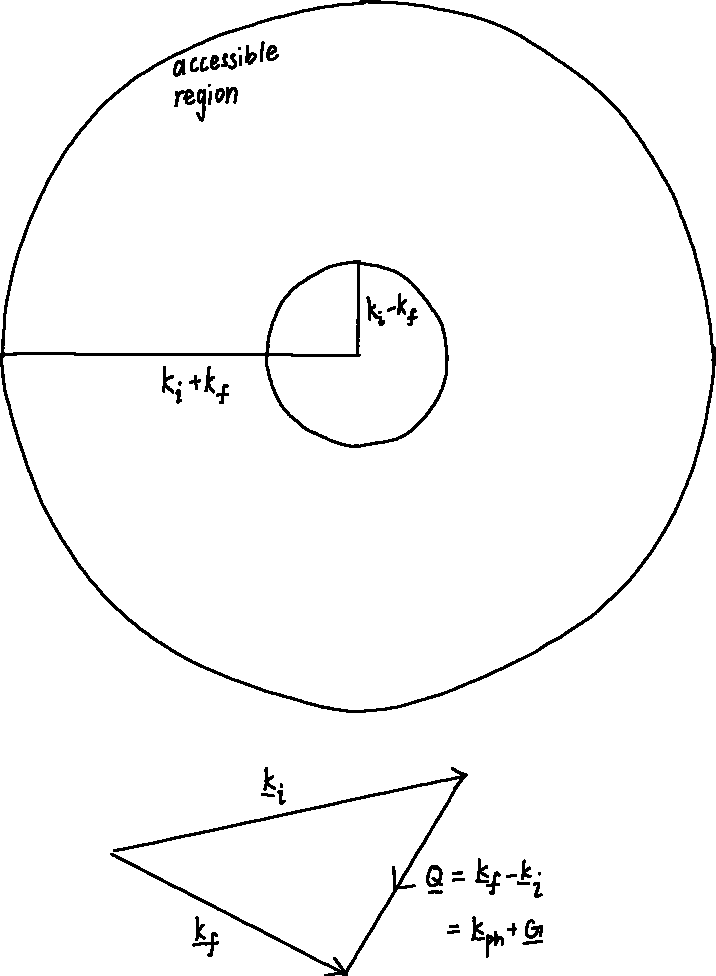
\includegraphics[width=.6\linewidth]{q6-ewald-sphere}
		\end{figure}
		
		It is clear that there exists a forbidden zone near the zone centre.
		Therefore to probe the forbidden zone, one must use the periodicity of reciprocal lattice to measure such zone in higher BZs.
		This may be done for $\mathbf{Q}$ with non-zero $\mathbf{G}$.
		\newpage
		\subpart \textbf{(TO BE VERIFIED)}
		Calculate $S(\mathbf{G})$ for 1st, 2nd and 3rd BZs.
		Then compare to see which yields the largest structure factor.
		
		By definition, we have the structure factor:
		\begin{align*}
			S(\mathbf{G}) &= \sum_{x \in \textnormal{UC}} b_x \mathrm{e}^{i \mathbf{G}\cdot\mathbf{R}_x} \\
			&= S_\textnormal{lattice} \times S_\textnormal{basis} \\
			&= \left( 1 + \mathrm{e}^{i\pi(h+k+l)} \right) \left[
			b_\textnormal{Ca}
			+ b_\textnormal{Fe} \left( \mathrm{e}^{i\pi(h+l/2)} - \mathrm{e}^{i\pi(h-l/2)} \right)
			+ b_\textnormal{As} \left( \mathrm{e}^{i\pi lz} - \mathrm{e}^{-i\pi lz} \right)
			\right] \\
			&= \left( 1 + \mathrm{e}^{i\pi(h+k+l)} \right) \left[ b_\textnormal{Ca}
			+ 2ib_\textnormal{Fe} \mathrm{e}^{i\pi h} \sin\left(\frac{l}{2}\right)
			+ 2ib_\textnormal{As} \sin\left(lz\right)
			\right]
		\end{align*}
		where $h$, $k$ and $l$ are the usual Miller indices.
		
		Enforcing $k=0$ and calculating the structure factor for each possible $\mathbf{G}$ then gives:
		\begin{gather*}
			S(\mathbf{G}) =
			\begin{cases*}
				0 \textnormal{\hspace{1em}for $h+l$ odd} \\
				2 b_\textnormal{Ca} \textnormal{\hspace{1em}}l=0 \\
				2 \left[ b_\textnormal{Ca} + 2ib_\textnormal{Fe} \sin\diagfrac{1}{2} + 2ib_\textnormal{As} \sin z \right] \textnormal{\hspace{1em}(1, 0, 1)} \\
				2 \left[ b_\textnormal{Ca} + 2ib_\textnormal{Fe} \sin 1 + 2ib_\textnormal{As} \sin\left(2z\right) \right] \textnormal{\hspace{1em}(0, 0, 2)}
			\end{cases*} \\
			|S(\mathbf{G})|^2 =
			\begin{cases*}
				0 \textnormal{\hspace{1em}for $h+l$ odd} \\
				\SI{88.36}{\femto\metre\squared} \textnormal{\hspace{1em}}l=0 \\
				\SI{88.61}{\femto\metre\squared} \textnormal{\hspace{1em}(1, 0, 1)} \\
				\SI{89.34}{\femto\metre\squared} \textnormal{\hspace{1em}(0, 0, 2)}
			\end{cases*}
		\end{gather*}
		
		Therefore to maximise the scattering intensity, one should probe the 3rd BZ.
	\end{subparts}
\end{parts}